\documentclass[fr]{../../../../../../eplexam}
\usepackage{../../../../../../eplchem}
\usepackage{../../../../../../eplunits}

\hypertitle{Chimie et chimie physique}{3}{FSAB}{1302}{2012}{Juin}
{Martin Braquet}
{Hervé Jeanmart, Christian Bailly et Francis Delannay}

\section{}

Soit la réaction irréversible d’ordre 2 : $A \Rightarrow B$. 

Une expérience est effectuée à 20$^\circ C$ avec une concentration initiale en réactif A non précisée (le produit B n’est pas présent au temps 0). La vitesse initiale de disparition de A est de $0,01 Mol/(L.min)$ et un quart du réactif disparaît en 5 minutes. 

A 30$^\circ C$, pour la même concentration initiale, c’est la moitié du réactif qui disparaît en 5 minutes.

Que vaut la concentration initiale en A, l’énergie d’activation et que vaut la constante de vitesse à 20$^\circ C$ et à 100$^\circ C$ ? (précisez les unités).

\begin{solution}

La loi de vitesse s'écrit:
$$r=k(T)[A]^2\Rightarrow \frac{1}{[A]}=\frac{1}{[A]_0}+k(T)t$$
On sait que
$$0,01=k(293K){[A]_0}^2$$
et
$$\frac{1}{3[A]_0/4}=\frac{1}{[A]_0}+5k(293K)$$
Cela constitue un système de 2 équations à 2 inconnues où
$$k(293K)= 0,4444 \:[L/(mol*min)]\qquad [A]_0=0,15 M $$
De la même manière,
$$\frac{1}{[A]_0/2}=\frac{1}{[A]_0}+5k(303K)$$
$$k(303K)= 1,333 \:[L/(mol*min)]$$
On calcule ensuite $E_a$:
$$\ln\frac{k(303K)}{k(293K)}=\frac{-E_a}{R}\bigg(\frac{1}{303}-\frac{1}{293}\bigg)$$
$$\Rightarrow E_a=-\ln\frac{k(303K)}{k(293K)}\frac{R}{\frac{1}{303}-\frac{1}{293}}=81176\:J/mol$$
Et on déduit enfin la constante de vitesse à 100$^\circ C$:
$$\ln\frac{k(373K)}{k(293K)}=\frac{-E_a}{R}\bigg(\frac{1}{373}-\frac{1}{293}\bigg)$$
$$\Rightarrow k(373K)=k(293K)\exp\bigg(\frac{-E_a}{R}\bigg(\frac{1}{373}-\frac{1}{293}\bigg)\bigg)=560,73\:[L/(mol*min)]$$

\end{solution}

\section{}

Montrez sur base de l’exemple ci-dessous, le lien entre la constante d’équilibre d’une réaction élémentaire équilibrée et la cinétique des réactions directe et inverse. 

Tirez-en le lien entre l’enthalpie de réaction et les énergies d’activation. 

Exprimez la loi de vitesse pour A sous forme différentielle si seul B est présent au temps 0.
$$2A\Longleftrightarrow B$$

\begin{solution}

Les vitesses de réaction directes et inverses sont:
$$r=k[A]^2 \qquad \mbox{et} \qquad r'=k'[B]$$
A l'équilibre, ces vitesse sont égales, on obtient alors
$$K=\frac{[B]}{[A]^2}=\frac{k}{k'}$$
On sait par ailleurs développer ces 2 expressions:
$$\exp\bigg(\frac{-\Delta G}{RT}\bigg)=\frac{A\exp\Big(\frac{-E_a}{RT} \Big)}{A'\exp\Big(\frac{-E_a'}{RT} \Big)}$$
$$\exp\bigg(\frac{S}{R}\bigg)\exp\bigg(\frac{-\Delta H}{RT}\bigg)=\frac{A}{A'}\exp\bigg(\frac{-(E_a-E_a')}{RT}\bigg)$$
$$\Rightarrow \Delta H=E_a-E_a'$$
avec $E_a$ et $E_a'$, les énergies d'activation des réactions directes et inverses.

On voit que deux moles de A donnent une mole de B:
$$[A]/2+[B]=\mbox{Cste}=[B]_0$$
On vérifie bien que s'il n'existe plus de B, on a $[A]/2=[B]_0$. Il y a donc 2 fois plus de moles de A que de B initialement.

Donc,
$$\frac{\mbox{d}[A]}{\mbox{d}t}=2r'-2r=2k'[B]-2k[A]^2=2k'\Big([B]_0-[A]/2 \Big)-2k[A]^2$$
On sait que l'on ne doit plus modifier cette équation différentielle puisque seul $[A]$ n'est pas constante. Il ne peut plus rester d'autres composés dont la concentration varie dans le temps.

\end{solution}

\section{}
\textit{Répondez succinctement aux trois questions suivantes. Ne pas
utiliser le verso de la feuille.}
\begin{itemize}
    \item Justifiez pourquoi l'enthalpie libre standard d'une réaction      chimique ne dépend ni de la pression du système réactionnel,         ni de sa composition.
    \item Expliquez pourquoi, selon la composition initiale du système        réactionnel, une réaction chimique peut, ou ne peut pas,            atteindre son état d’équilibre.
    \item Donnez les degrés d'oxydation des éléments dans la molécule de $H_2SO_4$.
\end{itemize}

\begin{solution}

\begin{itemize}
    \item Qualifier l’enthalpie d’une réaction de standard signifie dire qu’il s’agit de l’enthalpie de réaction à une pression de 1bar. Ce qui veut dire que l’enthalpie standard de réaction ne dépend pas de la pression. De plus l’enthalpie de réaction ne dépend pas de la composition du système car on peut l’écrire sous la forme suivante :
    $$\Delta H^\circ=\sum\limits_{i} \nu_i \Delta H^\circ_{f,i}$$ 
    \item On peut ne jamais atteindre l’équilibre si $\Delta \xi$ est borné dans un domaine où le minimum d’enthalpie libre de Gibbs n’est pas atteint.
    \item Les degrés d'oxydation de H et O sont +1 et -2, on déduit donc que celui de S est 6.
\end{itemize}

\end{solution}

\section{}

Une pile électrochimique fonctionnant à 25$^\circ C$ est constituée de deux électrodes. La première consiste en une tige de plomb baignant dans une solution de $Pb(NO_3)_2$ tandis que la seconde consiste en une tige d'argent plongée dans une solution de $AgNO_3$. Les potentiels standards de réduction de ces deux électrodes sont :
$$E^\circ_{Pb^{2+}/Pb}=-0,13V \qquad E^\circ_{Ag^{+}/Ag}=0,8V$$

\begin{enumerate}
    
\item  Ecrivez les deux demi-réactions ainsi que l'équation globale d'oxydo-réduction de cette pile.

\item  Dessinez-en le schéma en y indiquant l'anode, la cathode, et le sens de circulation des porteurs de charge.

\item  Quelle est la valeur de la force électromotrice standard de cette pile ?

\item  Quelle condition doit être remplie pour que la force électromotrice mesurée aux bornes de la pile soit égale à la force électromotrice standard ?

\item  Comment peut-on augmenter la force électromotrice de cette pile ?

\item  Calculez la valeur de la constante d'équilibre de la réaction globale d'oxydo-réduction.

\end{enumerate}

\begin{solution}

Cette question a été posée en janvier 2009.

\begin{solfig}{C}{Equilibre électro-chimique}
    \centering
    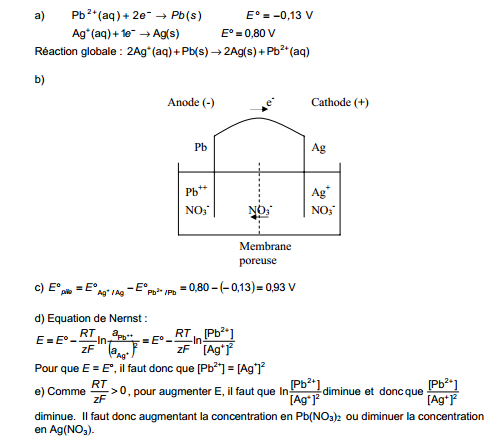
\includegraphics[scale=1]{Sol1.png}
\end{solfig}

\begin{solfig}{C}{Equilibre électro-chimique}
    \centering
    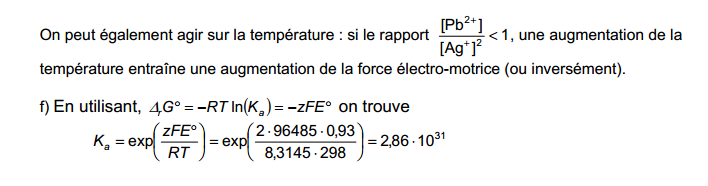
\includegraphics[scale=0.8]{Sol2.png}
\end{solfig}

\end{solution}

\section{}

On s'intéresse à la réaction suivante

$$2 HCN_{(g)} + 6 H_2O_{(g)} \Longleftrightarrow 2 {NH_3}_{(g)} + 3 {O_2}_{(g)} + 2 {CH_4}_{(g)}$$

On dispose des données thermodynamiques suivantes à 298K :

\begin{figure}[h]
    \centering
    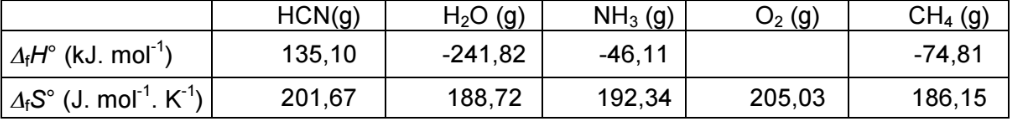
\includegraphics[scale=0.5]{Tab.png}
\end{figure}

\begin{enumerate}
    
\item Calculez $\Delta_r H^\circ(298K)$, $\Delta_r S^\circ(298K)$, et $\Delta_r G^\circ(298K)$. Justifiez le signe de $\Delta_r S^\circ(298K)$.

\item Calculez $K_p$ à 450$^\circ$C. Quelles hypothèses devez-vous faire pour permettre ce calcul ?

\item On introduit initialement dans le réacteur 3 moles de $HCN$ et 4 moles de $H_2O$. Montrez, sans effectuer les calculs, comment on pourrait calculer la composition du mélange et la pression du mélange à l'équilibre à n'importe quelle température si l'on connaît seulement la
température T et le volume V du réacteur.

\item Montrez par un exemple que le résultat obtenu au point 3 ne dépendrait pas de la manière dont l'équation (1) de la réaction a été écrite.

\end{enumerate}

\begin{solution}

\begin{enumerate}
    
\item 
    \begin{itemize}
    \item $\Delta_r H^\circ(298K)=938,8$ $[kJ/mol]$
    \item $\Delta_r S^\circ(298K)=-163,59$ $[J/(mol.K)]$, elle est négative car le nombre de moles des produits est inférieur au nombre de moles des réactifs.
    \item $\Delta_r G^\circ(298K)=987,629$ $[kJ/mol]$
    \end{itemize}

\item On fait l'hypothèse que les enthalpies et entropies de formation sont indépendantes de la température et que les gaz dans le réacteur ont les propriétés des gaz parfaits.
$$K(298K)=\exp\bigg(\frac{-\Delta G(298K)}{RT}\bigg)\simeq 0$$
En intégrant l'équation de van t'Hoff,
$$\ln\frac{K(723K)}{K(298)}=-\frac{\Delta H}{R}\bigg(\frac{1}{723}-\frac{1}{298}\bigg)$$
$$\Rightarrow K(723K)=K(298)\exp\bigg(\frac{-\Delta H}{R}\bigg(\frac{1}{723}-\frac{1}{298}\bigg)\bigg)=4,22*10^{-77}\simeq 0$$
Ce résultat laisse à penser que la réaction ne se déroulera pas et que la question trois n'a donc pas de sens physique.


\item Supposons néanmoins que la constante d'équilibre soit suffisamment grande, on peut alors trouver la composition du mélange par un tableau d'avancement de la réaction. 

On obtient ainsi ($n_{tot}=7-\xi$ et $p=(7-\xi)RT/V$):
$$K=\frac{(2\xi)^2(3\xi)^3(2\xi)^2}{(3-2\xi)^2(4-6\xi)^6}\frac{p^\circ V}{RT}$$
On obtient ainsi $\xi$ et on en déduit la pression totale en utilisant
$$ p=(7-\xi)RT/V .$$
\item Montrez par un exemple que le résultat obtenu au point 3 ne dépendrait pas de la manière dont l'équation (1) de la réaction a été écrite.

\end{enumerate}

\end{solution}

\section{}

Le cycle d’un moteur Stirling peut être approximé par les transformations réversibles suivantes :

\begin{itemize}
    \item 1 à 2 : compression isotherme 
    \item 2 à 3 : réchauffement isochore 
    \item 3 à 4 : détente isotherme 
    \item 4 à 1 : refroidissement isochore 
\end{itemize}

De telles machines utilisent usuellement de l'hélium (gaz idéal monoatomique, $M_m=4\:g/mol$). Les données connues sur l’une d’elles sont reprises dans le tableau ci-dessous. On sait également que le travail net fourni par le fluide et par cycle est de 4 kJ (soit $W=-4kJ$ selon les conventions de signe). Pour cette machine, 

\begin{enumerate}
    

\item Complétez le tableau suivant en justifiant succinctement vos résultats ;

\[
      \begin{tabular}{|c|cccc|}
        \hline
        & $p[\si{\bar}]$ & v[$m^3$] & $T[\si{\kelvin}]$ & $S-S_1[J/K]$\\
        \hline
        1 & 20 & 0,001 & 400 & 0\\
        \hline
        2 &  &  & 400 & \\
        \hline
        3 &  &  & 1100 & \\
        \hline
        4 &  &  & 1100 & \\
        \hline
      \end{tabular}
\]
\item Calculez la chaleur cédée à la source froide lors de la compression isotherme;

\item Calculez la puissance de la machine si la vitesse de rotation est de 1500 tours/minute (un tour = un cycle);

\item Calculez le rendement de ce cycle et commentez votre résultat en relation avec le rendement d'un cycle de Carnot travaillant aux mêmes températures. 

\item Quelle sera la puissance de la machine si, à défaut d’hélium,  on  utilise de l’azote tout en conservant les grandeurs connues du tableau  ci-dessus ? 

\end{enumerate}

\begin{solution}

\begin{enumerate}
    
\item
Voici les capacités calorifiques pour un gaz parfait monoatomique:
$$ c_p=\frac{5}{2}R \: [J/mol.K] \qquad c_v=\frac{3}{2}R\: [J/mol.K]$$
Le nombre de moles parcourant le cycle est 0,60136. On ajoute aussi que $V_4=V_1$.

On a donc
$$p_4=\frac{nRT_4}{V_4}=55\:[bar]$$
Le travail total s'exprime
$$W_{tot}=W_{1-2}+W_{3-4}=-\int_1^2 p\mbox{d}V-\int_3^4 p\mbox{d}V=-nR\bigg(T_1\ln\frac{V_2}{V_1}+T_3\ln\frac{V_4}{V_3}\bigg)$$
Et puisque $V_3=V_2$ et $V_4=V_1$,
$$-4000=-nR(T_1-T_3)\ln\frac{V_2}{V_1}$$
$$V_2=0,001\exp\bigg(\frac{4000}{8,3145*0,60136*(400-1100)}\bigg)=3,189*10^{-4}\:[m^3]$$
On complète trivialement le reste du tableau:
$$p_2=\frac{nRT_2}{V_2}=62,7143\:[bar]$$
$$p_3=\frac{nRT_3}{V_3}=172,4643\:[bar]$$
Et on termine avec les variations d'entropie,
$$S_2-S_1=\int_1^2\frac{\delta Q_{1-2}}{T}=\int_1^2\frac{-W_{1-2}}{T}=\int_1^2\frac{p\mbox{d}V}{T}=nR\ln\frac{V_2}{V_1}=-5,7143\: [J/K]$$
$$S_3-S_2=\int_2^3\frac{\delta Q_{2-3}}{T}=\int_2^3\frac{\mbox{d}U}{T}=\int_2^3\frac{C_v \mbox{d}T}{T}=C_v \ln\frac{T_3}{T_2}=12,6164\: [J/K]$$
$$S_4-S_3=\int_3^4\frac{\delta Q_{3-4}}{T}=\int_3^4\frac{-W_{3-4}}{T}=\int_3^4\frac{p\mbox{d}V}{T}=nR\ln\frac{V_4}{V_3}=5,7143\: [J/K]$$
$$S_1-S_4=\int_4^1\frac{\delta Q_{4-1}}{T}=\int_4^1\frac{\mbox{d}U}{T}=\int_4^1\frac{C_v \mbox{d}T}{T}=C_v \ln\frac{T_1}{T_4}=-12,6164\: [J/K]$$
Le tableau est complété ci-dessous:

\[
      \begin{tabular}{|c|cccc|}
        \hline
        & $p[\si{\bar}]$ & v[$m^3$] & $T[\si{\kelvin}]$ & $S-S_1[J/K]$\\
        \hline
        1 & 20 & 0,001 & 400 & 0\\
        \hline
        2 & 62,7143 & 0,0003189 & 400 & -5,7143\\
        \hline
        3 & 172,4643 & 0,0003189 & 1100 & 6,9021\\
        \hline
        4 & 55 & 0,001 & 1100 & 12,6164\\
        \hline
      \end{tabular}
\]

\item $Q_{1-2}=-W_{1-2}=\int_1^2p\mbox{d}V=nRT_1\ln\frac{V_2}{V_1}=-2286\:J$

\item $P=|W|V_{rot}=4000*1500/60=100kW$

\item 
Il ne faut pas prendre en considération les échanges de chaleurs qui ont lieu lors des échanges isochores dans le cas d'un moteur Stirling, car ceux-ci sont internes au système et ne font intervenir aucune source extérieur.
$$\eta=\frac{|W|}{Q_{HOT}}=\frac{|W|}{Q_{3-4}}=\frac{4000}{nRT_3\ln\frac{V_4}{V_3}}=0,64$$

Le rendement d'un cycle de Carnot est égal et vaut 
$$\eta_{Carnot}=1-\frac{T_2}{T_3}=0,64.$$


\item Le travail total vaut toujours 4000J et la puissance est donc identique.

\end{enumerate}

\end{solution}

\section{}

La présence nécessaire d’une source froide dans un cycle (tel celui de Carnot) est-elle une conséquence du second principe ? Argumentez judicieusement votre réponse.

Démontrez, à l’aide du concept d’entropie, le théorème de Carnot qui affirme qu’un "cycle réversible travaillant entre deux sources de chaleur à température constante a un rendement maximal".

\begin{solution}

Cela est expliqué aux pages 50-51 du syllabus de thermodynamique. En voici un passage: 

\textit{L’énoncé de Kelvin stipulait, en bref, qu’il est impossible de convertir totalement de la chaleur en travail. Imaginons que le bilan d’entropie interne puisse être négatif sur l’ensemble d’un cycle contrairement au constat fait ci-dessus. Dans ce cas, le bilan
d’entropie d’échange devrait être positif pour maintenir un bilan nul sur le cycle. On pourrait obtenir cela en ayant un apport unique d’une source chaude sans source froide. Par bilan d’énergie,
cet apport devrait être totalement transformé en travail. Cela est bien contraire à l’énoncé de Kelvin.
Réciproquement s’il était possible de convertir totalement de la chaleur en travail, il faudrait une
génération interne négative d’entropie ce qui est contradictoire au second principe.} 

\end{solution}

\end{document}
